\documentclass[13.5pt,aspecratio=169, xcolor=dvipsnames]{beamer}
\usepackage{graphicx} % Required for inserting images
\usepackage{subcaption}
\usepackage{amsfonts}
\usepackage{amsmath}
\usepackage{amssymb}
\usepackage{physics}
\usepackage{bm}
\usepackage{physics}
\usepackage{booktabs}
\usepackage{setspace}
\usepackage{xcolor}
\usepackage{wrapfig,lipsum}
\usetheme{Madrid}
\useinnertheme{circles}

\DeclareMathOperator*{\argmax}{arg\,max}
\DeclareMathOperator*{\argmin}{arg\,min}
\graphicspath{{Images/}{./}} 
\usetheme{Copenhagen}
\definecolor{UBCblue}{rgb}{0.04706, 0.13725, 0.26667} 
\usecolortheme[named=UBCblue]{structure}
%\usecolortheme{beaver}
\title{CHAPTER8: Vector Semantics and
Embeddings}
\author[CS221]{\textit{Instructor: PhD. Nguyen Thi Quy}\\ \bigskip \textbf{Group 5: 6.1 - 6.2}}
\date{\today}
\definecolor{mylightgreencolor}{RGB}{144, 238, 144}
\definecolor{mylightredcolor}{RGB}{255, 204, 203}
\setbeamertemplate{navigation symbols}{}
\setbeamertemplate{headline}{}
\setbeamercolor{huge text}{fg=white}
\setbeamertemplate{footline}{
    \leavevmode%
    \hbox{%
        \begin{beamercolorbox}[wd=.2\paperwidth,ht=2.25ex,dp=1ex,center]{author in head/foot}%
            \usebeamerfont{author in head/foot}\insertshortauthor
        \end{beamercolorbox}%
        \begin{beamercolorbox}[wd=.6\paperwidth,ht=2.25ex,dp=1ex,center]{title in head/foot}%
            \usebeamerfont{title in head/foot}\insertshorttitle
        \end{beamercolorbox}%
        \begin{beamercolorbox}[wd=.2\paperwidth,ht=2.25ex,dp=1ex,right]{date in head/foot}%
            \insertframenumber{} / \inserttotalframenumber\hspace*{2ex} 
        \end{beamercolorbox}%
    }%
    \vskip0pt%
}

\begin{document}
\maketitle

% \begin{frame}
% 	\frametitle{Table of Contents} % Slide title, remove this command for no title
% 	\tableofcontents[subsectionstyle=hide]
% \end{frame}
%-------------------------------------------------------------------%


\begin{frame}
    \doublespacing
        \frametitle{Presentation Overview} % Slide title, remove this command for no title
        
        \tableofcontents % Output the table of contents (all sections on one slide)
        %\tableofcontents[pausesections] % Output the table of contents (break sections up across separate slides)
\end{frame}
    
    %----------------------------------------------------------------------------------------
    %	PRESENTATION BODY SLIDES
    %----------------------------------------------------------------------------------------
    
    \section{Word Meaning} % Sections are added in order to organize your presentation into discrete blocks, all sections and subsections are automatically output to the table of contents as an overview of the talk but NOT output in the presentation as separate slides
    %------------------------------------------------
    \begin{frame}
        \doublespacing
            \frametitle{Presentation Overview} % Slide title, remove this command for no title
            
            \tableofcontents[currentsection] % Output the table of contents (all sections on one slide)
            %\tableofcontents[pausesections] % Output the table of contents (break sections up across separate slides)
    \end{frame}

%-------------------------------------------------------------------%

\begin{frame}
    \onehalfspacing
        \frametitle{What do words mean?}
        
        N-gram or text classification methods we've seen so far
        \begin{itemize}
            \item Words are just strings (or indices wi in a vocabulary list)
            \item That's not very satisfactory!
        \end{itemize}


        \begin{block}{Introductory logic classes:}
            The meaning of "dog" is \textbf{DOG}; cat is \textbf{CAT}
            \vspace{-3em}
            \begin{center}
                $$ \forall x, DOG(x) \longrightarrow MAMMAL(x) $$
            \end{center}
        \end{block}

        Old linguistics joke by Barbara Partee in 1967:
        \begin{itemize}
            \item \textbf{Q}: What's the meaning of life?
            \item \textbf{A}: LIFE
        \end{itemize}

        \begin{minipage}{0.37\textwidth}
            \begin{block}{}
                That seems hardly better!
            \end{block}
        \end{minipage}
    \end{frame}
    
    %--------------------------------------------------

    \begin{frame}
    \onehalfspacing
        \frametitle{Desiderata}
        {\Large
        What should a theory of word meaning do for us? \\
        \vspace{2em}
        Let's look at some desiderata \\
        \vspace{2em}
        From \textcolor{blue}{lexical semantics}, the linguistic study of word meaning}
    \end{frame}
    
    
    %------------------------------------------------
    \begin{frame}
        \onehalfspacing
            \frametitle{Lemmas and senses}
                \begin{figure}[h]
                    \centering
                    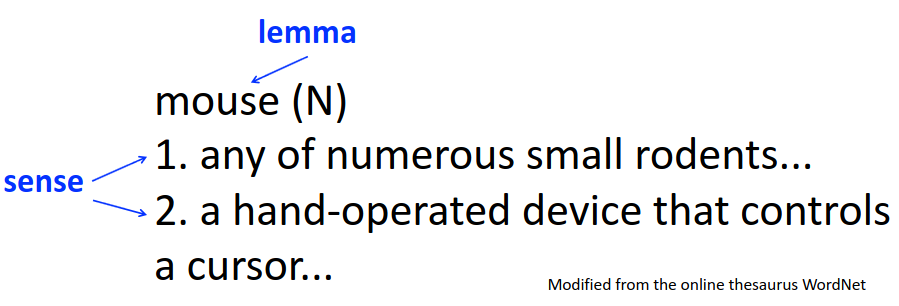
\includegraphics[width=\linewidth]{sense.png}
                \end{figure}
                
                {\large
                A \textcolor{blue}{sense} or \textcolor{blue}{“concept”} is the meaning component of a word
Lemmas can be \textcolor{blue}{polysemous} (have multiple senses) }
        \end{frame}
    
    %------------------------------------------------
    

\begin{frame}
\onehalfspacing
    \frametitle{Relations between senses: Synonymy}
    {\large
    Synonyms have the same meaning in some or all
contexts.

    \bigskip
    \begin{minipage}{0.45\textwidth}
    \begin{itemize}
        \item filbert / hazelnut
        \item couch / sofa
        \item big / large
    \end{itemize} 
    \end{minipage}
    \begin{minipage}{0.45\textwidth}
        \begin{itemize}
            \item automobile / car
            \item vomit / throw up
            \item water / $ \mathrm{H_2 O} $
        \end{itemize} 
    \end{minipage}
    
    }

\end{frame}
%------------------------------------------------


\begin{frame}
\onehalfspacing
    \frametitle{Relations between senses: Synonymy}
    {\large
    Note that there are probably no examples of perfect
synonymy.
    \begin{itemize}
\item Even if many aspects of meaning are identical
\item Still may differ based on politeness, slang, register, genre,
etc.
    \end{itemize}
    
    \bigskip
    \begin{minipage}{0.45\textwidth}
        \begin{block}{}
            \begin{center}
            water / $\mathrm{H_2 O}$ \\
            \vspace{-2em}
            \hspace{8em}\rule{0.5\textwidth}{0.4pt} \\
"$\mathrm{H_2 O}$" in a surfing guide?
            \end{center}
        \end{block}
    
    \end{minipage}
    \hspace{1em}
    \begin{minipage}{0.45\textwidth}
        \begin{block}{}
            \begin{center}
                big / large \\
            \vspace{-2em}
            \hspace{8em}\rule{0.5\textwidth}{0.4pt} \\
            my big sister $\ne$ my large sister
            \end{center}
        \end{block}
    
    \end{minipage}
    }

\end{frame}
%------------------------------------------------


\begin{frame}
    \onehalfspacing
        \frametitle{The Linguistic Principle of Contrast}
        {\LARGE
        \begin{center}
        Difference in form $\rightarrow$ difference in meaning
        \end{center}
        }
    
    \end{frame}
    %------------------------------------------------


\begin{frame}
    \onehalfspacing
        \frametitle{Abbé Gabriel Girard 1718t}
        \begin{minipage}{0.6\textwidth}
            \begin{minipage}{0.5\textwidth}
                \begin{block}{}
                    Re: "exact" synonyms
                \end{block}
                
            \end{minipage}
            \vspace{1em}


            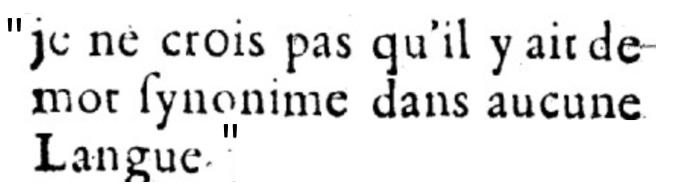
\includegraphics[width=\textwidth]{random_language.png}
            
            \vspace{1em}

            [I do not believe that there is a synonymous word in any language]

        \end{minipage}
        \begin{minipage}{0.35\textwidth}
            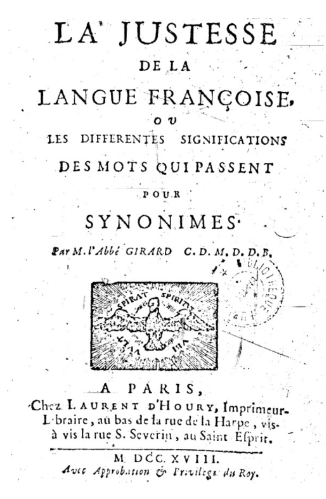
\includegraphics[width=\textwidth]{abbe.png}
        \end{minipage}
    \end{frame}
    %------------------------------------------------

    \begin{frame}
        \onehalfspacing
            \frametitle{Relation: \textbf{Similarity}}
            {\Large
            Words with similar meanings. Not synonyms, but sharing
some element of meaning
            \bigskip
            \begin{itemize}
                \item car, bicycle
                \item cow, horse
            \end{itemize}
            }
        \end{frame}
        %------------------------------------------------

        \begin{frame}
            \onehalfspacing
                \frametitle{Relation: \textbf{Similarity}}
                {\Large
                Ask humans how similar 2 words are}
                \bigskip
                
                \begin{figure}[h]
                    \centering

                    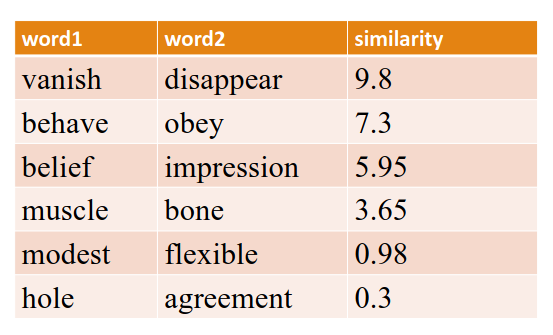
\includegraphics[width=0.8\textwidth]{words_similarity.png}
                    \captionsetup{labelformat=empty}
                    \caption{SimLex-999 dataset (Hill et al., 2015)}
                \end{figure}
            \end{frame}
            %------------------------------------------------

            \begin{frame}
                \onehalfspacing
                    \frametitle{Relation: Word relatedness}
                    {\Large
                    \begin{minipage}{0.53\textwidth}
                        \begin{block}{}
                            Also called "word association"
                        \end{block}

                        \bigskip

                    \end{minipage}

                    Words can be related in any way, perhaps via a semantic frame or field

                    \begin{itemize}
                        \item coffee, tea: \textbf{similar}
                        \item coffee, cup: \textbf{related}, not similar
                    \end{itemize}
                    }
                   
                \end{frame}
                %------------------------------------------------

                \begin{frame}
                    \onehalfspacing
                        \frametitle{Semantic field}
                        {\Large
                        \begin{block}{Words that:}        
                        \begin{itemize}
                            \item cover a particular semantic domain
                            \item bear structured relations with each other.
                        \end{itemize}
                    \end{block}
                        

                        \textbf{hospitals} \\
                        \hspace{1.3em} \textit{surgeon, scalpel, nurse, anaesthetic, hospital} \\
                        \textbf{restaurants} \\
                        \hspace{1.3em} \textit{waiter, menu, plate, food, menu, chef} \\
                        \textbf{houses} \\
                        \hspace{1.3em} \textit{door, roof, kitchen, family, bed}
                        }
                    \end{frame}
                    %------------------------------------------------

                    \begin{frame}
                        \onehalfspacing
                            \frametitle{Relation: Antonymy}
                            {\large
                            Senses that are opposites with respect to only one feature of meaning \\

                            \bigskip
                            Otherwise, they are very similar!

                            \textit{
                            \hspace{1.3em} dark/light \hspace{1.3em} short/long \hspace{1.3em} fast/slow \hspace{1.3em} rise/fall \\
                            \hspace{1.6em} hot/cold \hspace{1.3em} up/down \hspace{1.3em} in/out }
                            
                            \begin{block}{More formally: antonyms can}
                                \begin{itemize}
                                    \item Define a binary opposition or be at opposite ends of a scale: \\
                                    \begin{itemize}
                                        \item long/short, fast/slow 
                                    \end{itemize}
                                \item Be reversives: 
                                \begin{itemize}
                                \item rise/fall, up/down
                                \end{itemize}
                            \end{itemize}
                            \end{block}
                            }
                        \end{frame}
                        %------------------------------------------------

                        \begin{frame}
                            \onehalfspacing
                                \frametitle{Relation: Antonymy}
                                {\Large
                                Words have affective meanings
                                \begin{itemize}
                                    \item Positive connotations \textit{(happy)}
                                    \item Negative connotations \textit{(sad)}
                                \end{itemize}
    
                                \bigskip
                                \begin{block}{Connotations can be subtle:}
                                    \begin{itemize}
                                        \item Positive connotation: \textit{copy, replica, reproduction}
                                        \item Negative connotation: \textit{fake, knockoff, forgery}
                                    \end{itemize}
                                \end{block}
    
                                Evaluation (sentiment!)
                                \begin{itemize}
                                    \item Positive evaluation \textit{(great, love)}
                                    \item Negative evaluation \textit{(terrible, hate)}
                                \end{itemize}
                                }
                            \end{frame}
                            %------------------------------------------------
    
\begin{frame}
    \onehalfspacing
        \frametitle{Relation: Antonymy}
        \begin{block}{Words seem to vary along 3 affective dimensions:}
            \begin{itemize}
                \item \textbf{valence}: the pleasantness of the stimulus
                \item arousal: the intensity of emotion provoked by the stimulus
                \item dominance: the degree of control exerted by the stimulus
            \end{itemize}
        \end{block}

        \begin{figure}[h]
            \centering
            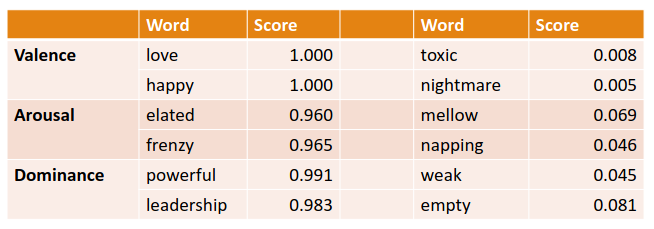
\includegraphics[width=\linewidth]{Antonymy.png}
            \captionsetup{labelformat=empty}
            \caption{Values from NRC VAD Lexicon (Mohammad 2018)}
        \end{figure}
    \end{frame}
    %------------------------------------------------
   
    \begin{frame}
        \onehalfspacing
            \frametitle{Word Meaning}
            {\Large
            \textbf{Concepts} or word senses
            \begin{itemize}
                \item Have a complex many-to-many association with \textbf{words} (homonymy,
                multiple senses)
            \end{itemize}
            Have relations with each other
                \begin{itemize}
                    \item Synonymy
                    \item Antonymy
                    \item Similarity
                    \item Relatedness
                    \item Connotation
                \end{itemize} }
        \end{frame}
        %------------------------------------------------
        \section{Vector Semantics}
        \begin{frame}
            \doublespacing
                \frametitle{Presentation Overview} % Slide title, remove this command for no title
                
                \tableofcontents[currentsection] % Output the table of contents (all sections on one slide)
                %\tableofcontents[pausesections] % Output the table of contents (break sections up across separate slides)
        \end{frame}
    
    %-------------------------------------------------------------------%
    \begin{frame}
        \onehalfspacing
            \frametitle{Computational models of word meaning}
            {\Large
            Can we build a theory of how to represent word
meaning, that accounts for at least some of the
desiderata?
            \bigskip
            \begin{block}{We'll introduce \textbf{vector semantics}}
                \begin{itemize}
                    \item The standard model in language processing!
                    \item Handles many of our goals!
                \end{itemize}
            \end{block}
}
        \end{frame}
        %------------------------------------------------

        \begin{frame}
            \onehalfspacing
                \frametitle{Ludwig Wittgenstein}
                {\Large
                PI \#43: \\
                
                \begin{minipage}{0.9\textwidth}
                    \begin{block}{}
                "The meaning of a word is its use in the language"
                    \end{block}
                \end{minipage}
                 }       
            \end{frame}
            %------------------------------------------------

            \begin{frame}
                \onehalfspacing
                    \frametitle{Let's define words by their usages}
                    {\large
                    One way to define "usage": \\

                    words are defined by their environments (the words around them)
                    
                    \vspace{1em}
                    
                        \begin{block}{Zellig Harris (1954):}
                            If A and B have almost identical environments we say that they
                            are synonyms.
                        \end{block}
                     }       
                \end{frame}
                %------------------------------------------------

\begin{frame}
    \onehalfspacing
        \frametitle{What does recent English borrowing \textit{ongchoi} mean?}
        Suppose you see these sentences:
        \begin{itemize}
            \item  Ong choi is delicious \textbf{sautéed with garlic.}
            \item Ong choi is superb \textbf{over rice}
            \item Ong choi \textbf{leaves} with salty sauces
        \end{itemize}

        And you've also seen these:
        \begin{itemize}
            \item …spinach \textbf{sautéed with garlic over rice}
            \item Chard stems and \textbf{leaves} are delicious
            \item Collard greens and other \textbf{salty} leafy greens
        \end{itemize}
        \begin{block}{Conclusion:}
            \begin{itemize}
                \item Ongchoi is a leafy green like spinach, chard, or collard greens
                \item We could conclude this based on words like "leaves" and "delicious" and "sauteed"
            \end{itemize}
        \end{block}
    \end{frame}
    %------------------------------------------------

\begin{frame}
\onehalfspacing
    \frametitle{Ongchoi: \textit{Ipomoea aquatica "Water Spinach"}}
    \begin{figure}[h]
        \centering
        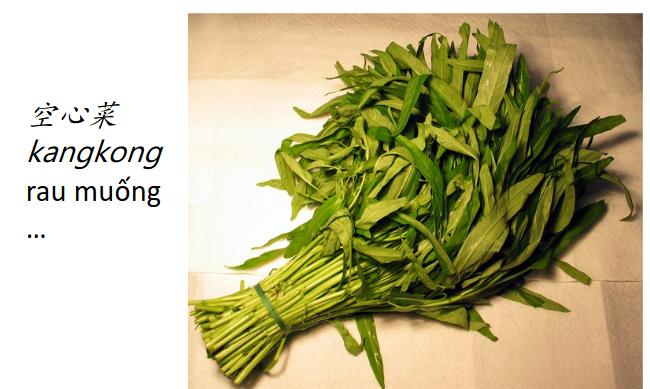
\includegraphics[width=\linewidth]{ongchoi.png}
    \end{figure}
\end{frame}
%------------------------------------------------

\begin{frame}
    \onehalfspacing
        \frametitle{Idea 1: Defining meaning by linguistic distribution}
        {\Large
        Let's define the meaning of a word by its
distribution in language use, meaning its
neighboring words or grammatical environments.
        }
    \end{frame}
    %------------------------------------------------

    \begin{frame}
        \onehalfspacing
            \frametitle{Idea 2: Meaning as a point in space (Osgood et al. 1957)}
            \begin{block}{3 affective dimensions for a word:}
                \begin{itemize}
                    \item \textbf{valence}: pleasantness
                    \item \textbf{arousal}: intensity of emotion
                    \item \textbf{dominance}: the degree of control exerted
                \end{itemize}
            \end{block}
            \begin{figure}[h]
                \centering
                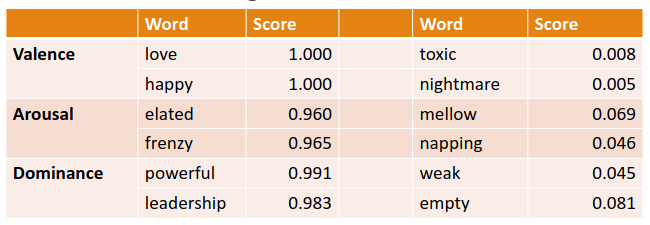
\includegraphics[width=\textwidth]{idea_2.png}
                \captionsetup{labelformat=empty}

            \end{figure}
                Hence the connotation of a word is a vector in 3-space
        \end{frame}
        %------------------------------------------------

        \begin{frame}
            \onehalfspacing
                \frametitle{Vector Semantics}
                {\Large
                Idea 1: Defining meaning by linguistic distribution

                \bigskip

                Idea 2: Meaning as a point in multidimensional space
                }
            \end{frame}
            %------------------------------------------------

\begin{frame}
    \onehalfspacing
        \frametitle{Defining meaning as a point in space based on distribution}
        {\Large
        Each word = a vector (not just "good" or $"w_{45}"$)

        \bigskip
        
        Similar words are \textbf{"nearby in semantic space"}

        \bigskip

        We build this space automatically by seeing which words are
        \textbf{nearby in text}
        \begin{figure}[h]
            \centering
            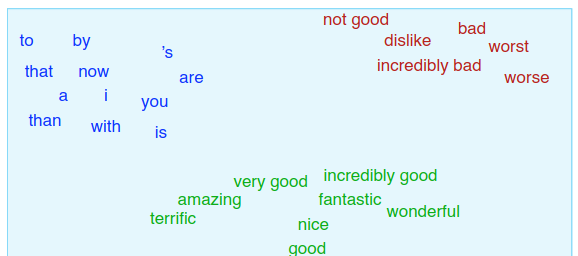
\includegraphics[width=0.8\linewidth]{word_vector.png}
        \end{figure}

        }
    \end{frame}
    %------------------------------------------------

    \begin{frame}
        \onehalfspacing
            \frametitle{We define meaning of a word as a vector}
            {\Large
            Called an "embedding" because it's embedded into a
space (see textbook)
    
            \bigskip
            \begin{block}{The standard way to represent meaning in NLP}
                Every modern NLP algorithm uses embeddings as
the representation of word meaning
            \end{block} 

            \bigskip

            Fine-grained model of meaning for similarity
    
            }
        \end{frame}
        %------------------------------------------------

\begin{frame}
    \onehalfspacing
        \frametitle{Intuition: why vectors?}
        {\large
        \begin{block}{Consider sentiment analysis:}
            \begin{itemize}
                \item With \textbf{words}, a feature is a word identity
                \item Feature 5: 'The previous word was "terrible"'
                \item requires \textbf{exact same word} to be in training and test 
            \end{itemize}
        \end{block}
        \begin{block}{With \textbf{embeddings}:}
            \begin{itemize}
                \item Feature is a word vector
                \item The previous word was vector [35,22,17…]
                \item Now in the test set we might see a similar vector [34,21,14]
                \item We can generalize to \textbf{similar but unseen} words!!! 
            \end{itemize}
        \end{block}


        }
    \end{frame}
    %------------------------------------------------

    \begin{frame}
        \onehalfspacing
            \frametitle{Intuition: why vectors?}
            We'll discuss 2 kinds of embeddings
            \begin{block}{Tf-idf}
                \begin{itemize}
                    \item Information Retrieval workhorse!
                    \item A common baseline model
                    \item \textbf{Sparse} vectors
                    \item Words are represented by (a simple function of) the \textbf{counts} of nearby words
                \end{itemize}
            \end{block}
            \begin{block}{Word2vec}
                \begin{itemize}
                    \item \textbf{Dense} vectors
                    \item Representation is created by training a classifier to \textbf{predict} whether a
                    word is likely to appear nearby
                    \item Later we'll discuss extensions called \textcolor{blue}{contextual embeddings}
                \end{itemize}
            \end{block}
    

        \end{frame}
        %------------------------------------------------



        \begin{frame}
            \onehalfspacing
                \frametitle{Computing with meaning representations}
                {\Large
                From now on:
Computing with meaning representations
instead of string representations}
                \begin{figure}[h]
                    \centering
                    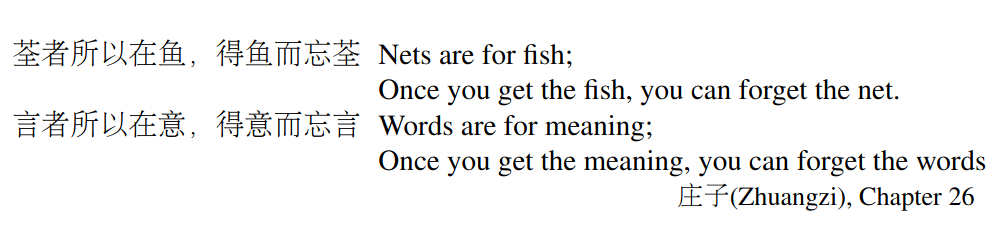
\includegraphics[width=\linewidth]{meaning_representations.png}
                \end{figure}
            
            \end{frame}
            %------------------------------------------------
                
            
        
    



\onehalfspacing
\begin{frame} % Use [allowframebreaks] to allow automatic splitting across slides if the content is too long
	\frametitle{Reference}
	
	\begin{thebibliography}{99} % Beamer does not support BibTeX so references must be inserted manually as below, you may need to use multiple columns and/or reduce the font size further if you have many references
		\footnotesize % Reduce the font size in the bibliography
		
		\bibitem[Stanford]{p1}
			Speech and Language Processing (3rd ed. draft)
			\newblock Dan Jurafsky and James H. Martin
			\newblock Part I: Fundamental Algorithms, \emph{Chapter 6: Vector Semantics and
            Embeddings}


	\end{thebibliography}
\end{frame}



%	CLOSING SLIDE
%----------------------------------------------------------------------------------------

\begin{frame} % The optional argument 'plain' hides the headline and footline
	\begin{center}
		{\Huge Thanks for listening!}
		
		\bigskip\bigskip % Vertical whitespace
		
		{\LARGE Q\&A section}
	\end{center}
\end{frame}
%------------------------------------------------


\end{document}
